%Note:
%   - Search XYZ: điền tên các bài báo về trích xuất sự kiện trên luật, template
%: ----------------------- introduction file header -----------------------
\chapter{Giới thiệu bài toán trích xuất sự kiện}

% the code below specifies where the figures are stored
\ifpdf
    \graphicspath{{1/figures/PNG/}{1/figures/PDF/}{1/figures/}}
\else
    \graphicspath{{1/figures/EPS/}{1/figures/}}
\fi

% ----------------------------------------------------------------------
%: ----------------------- introduction content -----------------------
% ----------------------------------------------------------------------


%: ----------------------- HELP: latex document organisation
% the commands below help you to subdivide and organise your thesis
%    \chapter{}       = level 1, top level
%    \section{}       = level 2
%    \subsection{}    = level 3
%    \subsubsection{} = level 4
% note that everything after the percentage sign is hidden from output




%: ----------------------- HELP: special characters
% above you can see how special characters are coded; e.g. $\alpha$
% below are the most frequently used codes:
%$\alpha$  $\beta$  $\gamma$  $\delta$

%$^{chars to be superscripted}$  OR $^x$ (for a single character)
%$_{chars to be suberscripted}$  OR $_x$

%>  $>$  greater,  <  $<$  less
%≥  $\ge$  greater than or equal, ≤  $\ge$  lesser than or equal
%~  $\sim$  similar to

%$^{\circ}$C   ° as in degree C
%±  \pm     plus/minus sign

%$\AA$     produces  Å (Angstrom)


%: ----------------------- HELP: references
% References can be links to figures, tables, sections, or references.
% For figures, tables, and text you define the target of the link with %\label{XYZ}. Then you call cross-link with the command \ref{XYZ}, as above
% Citations are bound in a very similar way with \cite{XYZ}. You store your %references in a BibTex file with a programme like BibDesk.





%\figuremacro{Ten file anh, dat trong figures}{A common glucose polymers}{The %figure shows starch %granules in potato cells, taken from %\href{http://molecularexpressions.com/micro/gallery/burgersnfries/burgersnfries4.html}{Molecular %Expressions}.}

%: ----------------------- HELP: adding figures with macros
% This template provides a very convenient way to add figures with minimal code.
% \figuremacro{1}{2}{3}{4} calls up a series of commands formating your image.
% 1 = name of the file without extension; PNG, JPEG is ok; GIF doesn't work
% 2 = title of the figure AND the name of the label for cross-linking
% 3 = caption text for the figure

%: ----------------------- HELP: www links
% You can also see above how, www links are placed
% \href{http://www.something.net}{link text}

%\figuremacroW{largepotato}{Title}{Caption}{0.8}
% variation of the above macro with a width setting
% \figuremacroW{1}{2}{3}{4}
% 1-3 as above
% 4 = size relative to text width which is 1; use this to reduce figures

%Intro here
%\pagestyle{plain}
\section{Động lực nghiên cứu}
\label{motivation}
\noindent \noindent Thế giới đang thay đổi rất nhanh  với sự tham gia của các phương tiện truyền thông xã hội. Mọi thông tin đều có thể đến với người dùng theo nhiều nguồn khác nhau. Tuy nhiên, sử dụng phương tiện truyền thông xã hội riêng lẻ khó có thể cập nhật được kịp thời và chính xác thông tin. Để đáp ứng nhu cầu đó, những hệ thống tổng hợp tin tức lần lượt ra đời giúp cho con người có thể dễ dàng nắm bắt thông tin. Khởi đầu bởi <tên hệ thóng đầu tiên trên thế giới>, tiếp sau đó là  <tên hệ thống khác 1>, <tên hệ thống khác 2>, \ldots Vào năm 2005, hệ thống tổng hợp tin tức tự động đầu tiên của Việt Nam ra đời dựa trên thành tựu nghiên cứu \emph{Hệ thống thu thập và tách thông tin ICPS} của hai tác giả Nguyễn Thành Long và Nguyễn Phú Bình đạt giải nhì cuộc thi Trí Tuệ Việt Nam 2002. \emph{Hệ thống xử lý tiếng Việt tự động ePi}  được người dùng biết đến với tên \textsc{Báo mới} \footnote{\href{www.baomoi.com}{www.baomoi.com}} và nhanh chóng trở thành trang tin tức tổng hợp được nhiều người sử dụng bởi tính tiện lợi và cập nhật. Mặc dù có những ưu điểm như vậy, một hệ thống tổng hợp tin tức vẫn có những yếu điểm chưa thể khắc phục. Thứ nhất, thông tin được thu thập từ những nguồn tin định trước dựa trên giao diện cập nhật của nguồn tin, chưa phân tích sâu về ý nghĩa và tính chất của sự kiện chứa đựng trong thông tin. Thứ hai, tin tức không được trực quan hóa theo xu hướng quan tâm của người dùng. Thông thường, độ ưu tiên quan tâm của người dùng là: thời gian (when) > địa điểm (where) >  thông tin gì(what). Hơn nữa, hệ thống tổng hợp tin tức xem xét tất cả các tin từ nguồn tin, sau đó phân lớp vào một lớp đã định nghĩa trước. Bởi tính phong phú của dạng thông tin, tính chính xác của quá trình phân lớp là một câu hỏi lớn chưa có lời giải đáp thỏa đáng! \\
\noindent Giải quyết nhược điểm của hệ thống tổng hợp tin tức tự động cần có một phương pháp trích xuất sự kiện phù hợp với tiếng Việt và hoạt động ổn định. Từ rất sớm, trích xuất sự kiện đã được cộng đồng khoa học máy tính đầu tư công sức nghiên cứu. Tiêu biểu có thể kể đến hội nghị \textbf{M}essage \textbf{U}nderstanding \textbf{C}onferences (MUC) \footnote{http://www-nlpir.nist.gov/related\_projects/muc}   tổ chức lần đầu tiên  năm 1987 dưới sự hỗ trợ của DARPA (Quỹ nghiên cứu bộ quốc phòng Hoa Kỳ). Một trong những đóng góp quan trọng của hội nghị MUC là đưa ra phương pháp trích xuất sự kiện theo khung  mẫu (\emph{scenario template}) với mục đích chính là lấy ra được sự kiện cùng các thông tin liên quan: tổ chức, đối tượng tham gia (người, sự vật, sự  việc). Độ chính xác và độ hồi tưởng của các nghiên cứu tham dự MUC nằm trong khoảng 50$\%$ tới 60 $\%$.
%Để cải tiến hiệu suất trích xuất, nhiều phương pháp trích xuất sự kiện dựa trên %luật ra đời như trong nghiên cứu của XYZ , ....
Ngoài ra, chương trình nâng cao hiệu quả trích xuất sự kiện \textbf{A}utomatic \textbf{C}ontent \textbf{E}xtraction (ACE) \footnote{http://projects.ldc.upenn.edu/ace} của Đại học Pennsylvania (Hoa Kỳ) cũng là một chương trình nổi tiếng, thu hút được nhiều nhóm nghiên cứu về trích xuất sự kiện tham gia và có những kết quả rất tích cực. Tuy nhiên, trích xuất sự kiện là một vấn đề mang đặc trưng ngôn ngữ học. Ngôn ngữ ảnh hướng rất lớn tới hiệu quả của một phương pháp trích xuất. Theo tìm hiểu của chúng tôi, trích xuất sự kiện trên dữ liệu tiếng Việt chưa có nhiều nghiên cứu. Bởi vậy, phương pháp trích xuất sự kiện dành cho tiếng Việt vẫn còn hạn chế cả về chất lượng lẫn số lượng.

%Defense Advanced Research Project Agency, United States of America
\\
\noindent Một yếu tố khác đưa chúng tôi đến với đề tài nghiên cứu này là sự thú vị trong xử lý dữ liệu lớn. Theo xu hướng phát triển Công Nghệ Thông Tin hiện đại, thi hành hệ thống với dữ liệu lớn là tất yếu. Các công ty hàng đầu thế giới về Công Nghệ như Microsoft \footnote{www.microsoft.com}, Google \footnote{www.google.com}, Oracle \footnote{www.oracle.com}, Facebook \footnote{www.facebook.com} đều có những chiến lược phát triển lâu dài về xử lý dữ liệu lớn. Cùng với đó, những trường đại học hàng đầu thế giới về khoa học máy tính đều đưa vào trường trình đào tạo của mình khoa học về xử lý dữ liệu lớn như Đại học Priceton \footnote{http://www.cs.princeton.edu/courses/archive/spr02/cs493} (Hoa Kỳ) , Đại học Stanford \footnote{http://www.stanford.edu/class/cs246} (Hoa Kỳ) , Đại học Carnegie Mellon \footnote{http://www.cs.cmu.edu/~neill/courses/90866.html} (Hoa Kỳ) hay Đại học tổng hợp Zurich \footnote{\href{http://las.ethz.ch/courses/datamining-s12}{http://las.ethz.ch/courses/datamining-s12}} (Thụy Sỹ). Sự hỗ trợ tuyệt vời về dữ liệu và kỹ thuật  từ phía ThS. Trần Mai Vũ đã giúp chúng tôi có thêm động lực và quyết tâm hoàn thành đề tài.



\section{Vấn đề nghiên cứu}
\label{problem}
    \subsection{Bài toán}
    \noindent Những vấn đề phân tích ở phần \ref{motivation} đã đưa nhóm nghiên cứu hướng tới ý tưởng đưa ra phương pháp trích xuất sự kiện phù hợp khi xử lý với dữ liệu tiếng Việt và xây dựng nên một hệ thống theo dõi tin tức trực tuyến mà trong đó trích xuất sự kiện là yếu tố trung tâm. Nghiên cứu đóng góp ở cả hai nội dung: khoa học và ứng dụng. Ý nghĩa của việc giải quyết vấn đề này được trình bày chi tiết ở mục \ref{meaning}.
\paragraph{Đầu vào} của bài toán là một bản ghi tin tức về một trong  ba lĩnh vực: tai nạn giao thông, hình sự, cháy nổ. Mỗi bản ghi bao gồm các thông tin: tiêu đề, tóm tắt nội dung, toàn văn tin tức. Gần 4 triệu \footnote{3.842.137 bài báo tin tức tổng hợp được thu thập trong 1 tháng, từ 01/12/2011 đến 01/01/2012 sử dụng bộ CRAWLER của tác giả Trần Mai Vũ} tin tức thu thập từ trang các nguồn cung cấp tin tức (phụ lục \ref{website}) thông qua trang tổng hợp tin tức \textsc{Báo mới} \footnote{\href{www.baomoi.com}{www.baomoi.com}} là lượng dữ liệu mà hệ thống sẽ sử dụng.

\paragraph{Kết quả mong muốn} của bài toán là có hay không có sự kiện trong bản ghi tin tức. Nếu có thì phải đưa ra được các thông tin liên quan tới sự kiện gồm có: tên sự kiện, thời gian, địa điểm, người, sự vật, sự việc. Sự kiện thu được cũng phải được trực quan hóa trên hệ thống theo dõi tin tức trực tuyến.
\paragraph{Vậy, sự kiện là gì?} Theo Allan, tin tức được cho là phản ánh một sự kiện nếu nó có đủ bốn yếu tố:  hành vi, chủ thể, thời gian, địa điểm \cite{JRV98}. Hành vi là các hoạt động/hành động gây ra sự kiện. Chủ thể có thể là con người, sự vật hoặc sự việc. Cũng theo công bố này, để định nghĩa rõ ràng thế nào là sự kiện rất khó bởi tính nhập nhằng liên quan tới các yếu tố ngữ cảnh, ngôn ngữ, văn hóa. Ví dụ, \emph{Chiều ngày \texttt{5/3/2012}, tai nạn giao thông tại \texttt{ngã tư Khuất Duy Tiến} làm \texttt{2 người} tử vong} là một sự kiện nói về tai nạn giao thông. Nhưng \emph{Theo báo cáo của cảnh sát giao thông \texttt{Hà Nội} \texttt{chiều nay}, số \texttt{người} chết vì tai nạn giao thông giảm 30\% so với cùng kỳ năm ngoái} lại không phải là một sự kiện dù có đủ 3 yếu tố kể trên. Trong phạm vi giải quyết bài toán trích xuất sự kiện, việc định nghĩa rõ ràng sự kiện mà nghiên cứu quan tâm luôn là yêu cầu trước tiên. Ban đầu  hội nghị MUC chỉ quan tâm các sự kiện về hoạt động quân sự. Sau đó, tới lần tổ chức thứ 3 mở rộng thêm các sự kiện về khủng bố, đầu tư mạo hiểm, tai nạn máy bay, \ldots Các thuộc tính cần phải có của một sự kiện mà MUC yêu cầu gồm có: tác nhân, thời gian, địa điểm và các tác động của nó. Ở chương trình ACE, sự kiện được định nghĩa là một hoạt động nào đó do các đối tượng tham gia tạo nên. Một cách đơn giản, sự kiện là một sự thay đổi trạng thái. Bên cạnh đó, dạng sự kiện và các thuộc tính về sự kiện được quy định chặt chẽ hơn với tám dạng sau: LIFE (sự sống--chết), MOVEMENT (sự di chuyển), TRANSACTION (giao dịch), BUSINESS (kinh tế), CONFLICT (xung đột), CONTACT (giao thiệp, gặp gỡ), PERSONNEL (nhận--đuổi việc), JUSTICE (pháp lý). Mỗi dạng sự kiện lại có phân biệt từng dạng con. Ví dụ như LIFE có các dạng  sự kiện  con BE-BORN (chào đời), INJURE (bị thương), DIE (chết) hay PERSONNEL có START--POSITION (vị trí khi nhận việc), END--POSITION (vị trí trước khi bị thôi việc), NOMINATE (bổ nhiệm), ELECT (bầu chọn), \ldots
\\
\noindent Hầu hết những nghiên cứu được trích dẫn trong báo cáo này đều chỉ tập trung vào một lĩnh vực cụ thể. \cite{MM09}, \cite{YKW09} khai thác các sự kiện trên trang cá nhân.  \cite{CVJ09}, \cite{CHR04} tập trung vào sự kiện y sinh học. \cite{HJM08}, \cite{JHP07} thực hiện trích xuất sự kiện thảm họa, mối nguy hiểm đe dọa. Ngoài ra, sự kiện về giải thưởng Nobel \cite{FHH06}, sự kiện về chứng khoán \cite{FHD02}, sự kiện về đầu tư tài chính \cite{CM00} hay các sự kiện về chính trị \cite{FK08}, \cite{CM00} cũng được quan tâm. Nghiên cứu này thực hiện trích xuất sự kiện từ các bản tin thông báo hằng ngày cho các loại sự kiện nói về tai nạn giao thông, các vi phạm hình sự, các vụ cháy nổ. Một cách tường minh,  sự kiện được định nghĩa  rằng phải có đủ ba thuộc tính: chủ thể, thời gian và địa điểm và bắt buộc thuộc ba dạng: TAI NẠN GIAO THÔNG, HÌNH SỰ, CHÁY NỔ.

\paragraph{Thế nào là trích xuất sự kiện?} Trước hết, trích xuất sự kiện là một lĩnh vực con thuộc trích chọn thông tin (Information Extraction). Tự động nhận biết và tách được thông tin về sự kiện trong các tài liệu không có cấu trúc là định nghĩa tổng quát nhất về trích xuất sự kiện. Chi tiết hơn, trích xuất sự kiện tập trung nhận dạng sự kiện thuộc một miền lĩnh vực cụ thể biết trước, đồng thời đưa ra được tập các tham số--là các thông tin xung quanh sự kiện đó, bao gồm: tác nhân, thời gian, địa điểm, \ldots Trong \cite{RG10}, Grishman cho rằng trích xuất sự kiện là một bài toán khó, bởi gặp nhiều vấn đề về xử lý ngôn ngữ tự nhiên cũng như khảo sát dữ liệu rất mất thời gian.


\subsection{Các vấn đề cần giải quyết}
 \noindent Nghiên cứu sẽ trả lời ba câu hỏi.
 \begin{description}
 \item[Thứ nhất] thế nào là trích xuất sự kiện tin tức và những phương pháp thường được sử dụng để làm điều đó?
\item[Thứ hai] tồn tại những khó khăn nào  khi áp dụng những phương pháp từ câu hỏi trên vào dữ liệu tiếng Việt và cách giải quyết những khó khăn này?
\item[Và cuối cùng] một hệ thống theo dõi tin tức có khả thi không?
 \end{description}

\section{Ý nghĩa}
    \label{meaning}
    \subsection{Ý nghĩa khoa học}

\noindent Về mặt khoa học, chúng tôi đề xuất phương pháp trích xuất sự kiện dựa trên luật ngữ nghĩa kết hợp với học máy để thu được sự kiện xảy ra hằng ngày thông qua  dữ liệu tin tức tiếng Việt thu thập từ một số nguồn thông tin tin cậy dưới sự cho phép của Bộ Thông Tin và Truyền Thông \footnote{\href{http://mic.gov.vn/vbqppl/Lists/Vn$\%$20bn$\%$20QPPL/DispForm.aspx?ID=6988}{http://mic.gov.vn/vbqppl/Lists/Luat-cong-nghe-thong-tin}}(xem danh sách trang báo điện tử cung cấp tin tức tại  phụ lục \ref{website}, trang \pageref{website}). Luật ngữ nghĩa và học máy Maximum Entropy đều là những phương pháp đã được sử dụng trong các công bố quốc tế như \cite{CVJ09}, \cite{RDA05}, \cite{MD04}. Mỗi phương pháp đều có những ưu, nhược điểm riêng. Để nâng cao hiệu quả trích xuất và rút ngắn thời gian thực hiện, kết hợp hai phương pháp trên là cách tiếp cận hợp lý. Tuy nhiên trên thế giới chưa có nghiên cứu nào đi theo hướng tiếp cận này.
\\ \noindent Trong bối cảnh vấn đề trích xuất sự kiện ở trong nước chưa có nhiều nghiên cứu, công trình của chúng tôi sẽ góp phần thôi thúc đề tài thú vị này được quan tâm nhiều hơn bởi lẽ đây là vấn đề tương đối mới mẻ, có khả năng ứng dụng thực tiễn cao và còn rất nhiều lĩnh vực cần quan tâm. Một số ví dụ như sự kiện Y--SINH, sự kiện KINH TẾ--ĐẦU TƯ, sự kiện CHÍNH TRỊ.

\subsection{Ý nghĩa thực tiễn}
\noindent Xét tới  phương diện  ứng dụng, chúng tôi tiến hành xây dựng một hệ thống theo dõi thông tin trực tuyến. Như đã nói ở mục \ref{motivation}, một hệ thống tổng hợp tin tức tự động chưa đủ thông minh để đáp ứng nhu cầu ngày càng cao của người dùng. Bởi thế, trong nghiên cứu này chúng tôi muốn xây dựng một hệ thống theo dõi, giám sát thông tin sự kiện. Bởi quy mô của một công trình sinh viên nghiên cứu khoa học, nhóm chúng tôi tập trung vào ba loại sự kiện thường xảy ra hằng ngày: tai nạn giao thông, hình sự và cháy nổ. Một cách rõ ràng nhất, sự kiện thuộc ba dạng trên sẽ được trích xuất theo các thông tin: tên sự kiện, thời gian/địa điểm diễn ra sự kiện, các nhân tố tham gia sự kiện. Sau đó, sự kiện được trực quan hóa trên  bản đồ giúp cho người sử dụng dễ dàng theo dõi. Theo khảo sát của nhóm nghiên cứu, một hệ thống như đã mô tả chưa xuất hiện ở Việt Nam. Đề tài nghiên cứu đóng góp vào việc phổ biến hình thức nắm bắt tin tức mới dễ dùng và trực quan hơn so với các hệ thống cung cấp tin tức truyền thống.


 \section{Thách thức}
   \noindent  Mặc dù được các nhà khoa học quan tâm nghiên cứu  từ rất sớm, trích xuất sự kiện vẫn còn những khó khăn cần phải vượt qua. \\
\noindent Trích xuất sự kiện liên quan mật thiết tới các nghiên cứu về ngôn ngữ học. Lĩnh vực xử lý ngôn ngữ tự nhiên nói chung và xử lý tiếng Việt nói riêng tương đối rộng, tồn tại nhiều bài toán chưa được giải quyết triệt để mà trong đó có  xử lý nhập nhằng ngữ nghĩa (Word Sense Disambiguation), bài toán đồng tham chiếu (Co--references) hay việc nhận dạng tính đa hình cấu trúc ngữ pháp trong tiêu đề tin tức (Syntactically  Ambiguous Headlines). Ba bài toán trên là những khó khăn cơ bản nhất mà chúng tôi phải giải quyết để đưa ra được phương pháp trích xuất sự kiện phù hợp.

\\
\noindent Tính tới thời điểm thực hiện công trình, Việt Nam chưa có nghiên cứu nổi bật về trích xuất sự kiện. Bởi vậy, nhóm nghiên cứu không được kế thừa những công trình, những kinh nghiệm khi thực hiện với dữ liệu tiếng Việt. Nhóm cần nhiều thời gian hơn để thử nghiệm và đánh giá phương pháp nào là tốt, phù hợp với mục tiêu đề ra.
\\
\noindent Ngoài ra, khó khăn trong xử lý dữ liệu lớn cũng là một thách thức mà nhóm nghiên cứu phải đối mặt. Để có thể trích chọn được sự kiện từ tập dữ liệu lớn cần phải tối ưu thuật toán đảm bảo rằng hệ thống có thể hoạt động tốt trong điều kiện tài nguyên cho phép.


\section{Nghiên cứu liên quan}
	\subsection{Một số nghiên cứu liên quan ở nước ngoài}
% NLDB \footnote{\href{http://www.nldb.org/}{International conference on
%Applications of Natural Language Processing
%to Information Systems}},
\noindent Kể từ hội nghị MUC lần đầu tiên (1987) cho tới nay, hàng ngàn nghiên cứu về trích xuất sự kiện đã được công bố trong những  hội nghị, chương trình có uy tín cao như MUC, SIGKDD \footnote{\href{http://www.kdd.org/}{International Conference on \textbf{K}nowledge \textbf{D}iscovery and \textbf{D}ata Mining}} , ACM SIGIR \footnote{\href{http://www.sigir.org/}{\textbf{S}pecial \textbf{I}nterest \textbf{G}roup on \textbf{I}nformation \textbf{R}etrieval}}, TDT \footnote{\href{http://projects.ldc.upenn.edu/TDT/}{\textbf{T}opic \textbf{D}etection and \textbf{T}racking}}, ACE. Theo Hogenboom. F và các cộng sự, tựu chung lại các công bố này có thể phân loại theo ba hướng tiếp cận chính: phân tích ngữ nghĩa (còn gọi là hướng theo nội dung), học máy--thống kê (hướng theo dữ liệu) và cuối cùng là kết hợp hai  cách tiếp cận trên \cite{FFU11}.
\\
\noindent Giai đoạn cuối thập niên tám mươi, đầu thập niên chín mươi, sự kiện được trích xuất chủ yếu dựa trên các mẫu được tạo sẵn (\emph{scenario template}) \cite{BS92}. Mẫu là các bản ghi còn thiếu thông tin sự kiện. Thông tin về sự kiện còn thiếu  này sẽ được bổ sung từ dữ liệu căn cứ vào những thông tin đã định nghĩa trên mẫu. Một cách thuần túy thì đây là bài toán tìm kiếm các từ được định nghĩa trước rồi lấy thông tin đi kèm với chúng để điền vào mẫu. Độ chính xác của phương pháp này ở mức trung bình nằm trong khoảng 50$\%$--60$\%$ \cite{MW11}. Cách giải quyết bài toán hết sức đơn giản mà về sau, trong các chương trình nghiên cứu TDT hay ACE vẫn còn sử dụng nhưng với những định nghĩa mẫu tổng quát và trên nhiều miền lĩnh vực khác nhau. Hơn nữa, đây cũng là sự khởi đầu của các phương pháp đi theo hướng tiếp cận đầu tiên kể ở trên: sử dụng luật phân tích ngữ nghĩa.
\\
\noindent Trong nghiên cứu của Nishihara và cộng sự, ba thông tin: địa điểm, đối tượng, hành vi  của  sự kiện được lấy ra từ trang cá nhân \footnote{\emph{blog}} \cite{YKW09} sử dụng các \emph{luật lexico--syntactic} \footnote{\emph{Luật lexico--syntactic} là sự kết hợp giữa biểu thức chính quy với từ vựng thuộc miền lĩnh vực và các quy tắc ngữ pháp của ngôn ngữ để sinh luật} để tìm kiếm các câu chứa sự kiện trong từng bài viết \footnote{\emph{entry}}. Cùng với cách tiếp cận này, Aone.C và Ramos.M đã trích chọn các sự kiện về tài chính và chính trị. Hai tác giả tập trung đưa ra các luật biểu diễn quan hệ giữa sự kiện với các thông tin xung quanh nhằm mục đích khai thác tối đa thuộc tính của sự kiện, và giữa các sự kiện để lấy được tập các sự kiện liên quan tới nhau \cite{CM00}. Nghiên cứu của Xu và cộng sự cũng sử dụng các \emph{luật lexico--syntactic} trên dữ liệu bản tin về sự kiện giải thưởng Nobel. Nhưng thay vì các luật được áp dụng ngay trên dữ liệu, một tập luật được tạo ra sau đó sử dụng học máy không giám sát để huấn luyện tập luật này trên  tập các bản tin đã được gán nhãn.
Sau đó mô hình học sẽ được áp dụng với các bản tin còn lại \cite{FHH06}. \\
\noindent Một điểm yếu của \emph{luật lexico--syntactic} là không thể phủ hết được trạng thái quan hệ giữa các sự kiện, có nghĩa là không thể nhận biết hai sự kiện có trùng nhau hay không. Do đó, giám sát quá trình tiến triển của một sự kiện là tương đối khó khi sử dụng cách tiếp cận này. Nhằm khắc phục điều này, \emph{luật lexico--semantic} \footnote{\emph{luật lexico--semantic} là sự kết hợp giữa biểu thức chính quy, tập từ vựng thuộc miền lĩnh vực và vai trò ngữ nghĩa của từ vựng trong ngôn ngữ để sinh luật} được đề xuất. Nghiên cứu của Li và đồng nghiệp chú trọng đưa ra các luật lấy sự kiện về giá cổ phiếu qua các bản tin chứng khoán \cite{FHD02}. Một tập dữ liệu bản tin chứng khoán được gán nhãn bởi từ điển ngữ nghĩa chứa tên  công ty, tập đoàn mà phần nhiều là tên vị trí địa lý. Ngoài ra, lĩnh vực y sinh cũng được nhiều nhà nghiên cứu quan tâm. Nghiên cứu của nhóm do Cohen chủ trì tập trung xây dựng bộ trích xuất nội dung có nhiệm vụ trích chọn sự kiện y tế bằng từ điển thuật ngữ y sinh và quan tâm tới nghĩa của các cụm từ \cite{CVJ09}. Cùng sử dụng cách làm này, Vargas--Vera và Celjuska đã phát triển hệ nhận dạng sự kiện trên các bài báo của Knowledge Media Institute \footnote{\href{http://kmi.open.ac.uk/}{http://kmi.open.ac.uk/}} \cite{MD04}.\\
\noident Những phương pháp đã trình bày ở trên chủ yếu xây dựng luật dựa trên tri thức về ngôn ngữ. Chúng có một số lợi điểm có thể kể tới. Thứ nhất, thông tin muốn có được hoàn toàn có thể theo ý định của người nghiên cứu, và trên bất cứ lĩnh vực cụ thể nào. Thứ hai, không cần phải xem xét một tập dữ liệu quá lớn. Một luật chủ yếu dựa trên tri thức ngôn ngữ và sự khảo sát của người thực hiện. Tuy nhiên, các  phương pháp này cũng có những điểm yếu cần phải khắc phục. Bởi luật được sinh ra cho từng dạng sự kiện cụ thể nên chúng ta không thể sử dụng lại luật cho trường hợp khác. Nếu trích xuất sự kiện trong lĩnh vực rộng thì áp dụng luật không thể bao quát toàn bộ không gian dữ liệu. Hơn nữa, việc khảo sát và sinh luật bằng tay là một công việc rất mất thời gian và tẻ nhạt. Cách tiếp cận hướng dữ liệu sẽ cho chúng ta một cái nhìn cụ thể hơn khi giải quyết những vấn đề tồn đọng của phương pháp tiếp cận hướng nội dung.
\\
\noindent Đối với  cách tiếp cận hướng dữ liệu, các nhà nghiên cứu thường sử dụng các phương pháp học máy: học giám sát (SVM), học bán giám sát, học không giám sát (phân cụm) hay là các  phương pháp thống kê như trọng số IF--IDF. Năm 2009, Okamoto cùng cộng sự xây dựng một hệ thống phát hiện và trích xuất sự kiện trong một phạm vi địa lý sử dụng kỹ thuật  phân cụm phân cấp với dữ liệu là các bài viết trên trang cá nhân \footnote{blog} \cite{MM09}. Phân cụm cũng là kỹ thuật được sử dụng nhiều trong các nghiên cứu khác như công trình của nhóm  Liu \cite{MYL08}, nhóm Tanev \cite{HJM08}. Ở công trình thứ nhất, một cụm sự kiện liên quan tới tin tức hằng ngày  hình thành sẽ được sắp xếp theo thứ tự nhờ sử dụng đồ thị vô hướng phân đôi. Công trình thứ hai lại sử dụng một tập dữ liệu đã được gán nhãn tự động để phân cụm sự kiện nói về mối nguy hiểm, thảm họa. Phương pháp máy vector hỗ trợ \footnote{Support Vector Machine} được Lei và cộng sự thử nghiệm trên hệ thống phát hiện sự kiện tin tức của họ \cite{LWZ05}. Brants và cộng sự cải tiến cách tính  trọng số TF--IDF để nhận dạng một sự kiện thông qua một sự kiện khác đã biết. Độ tương đồng giữa hai sự kiện quyết định bởi hai yếu tố: độ tương đồng giữa từ khóa của hai bản tin, độ tương đồng giữa hai nguồn cung cấp bản tin \cite{TFA03}. Tiếp cận hướng dữ liệu vẫn còn tồn tại một số nhược điểm: không quan tâm đến ngữ nghĩa, và lượng dữ liệu phải khá lớn. Hướng tiếp cận này không thể nào trích xuất được quan hệ giữa các sự kiện cũng như quan hệ giữa các thuộc tính của sự kiện. Bởi sử dụng chủ yếu các phương pháp học máy, thống kê nên dữ liệu cần thiết là khá lớn. Xây dựng được kho dữ liệu đủ lớn cũng là một yêu cầu không đơn giản.
\\
\noindent Như những dẫn chứng ở trên, cả hai cách tiếp cận hướng nội dung và hướng dữ liệu đề có những điểm mạnh và điểm yếu riêng. Một cách tự nhiên, kết hợp hai cách tiếp cận này với nhau sẽ giúp chúng hỗ trợ, bổ xung cho nhau. Nghiên cứu của Jungermann và Morik kết hợp \emph{luật lexico--syntactic} với trường điều kiện ngẫu nhiên \footnote{Conditional Random Fields} để trích xuất sự kiện từ văn bản các phiên họp toàn thể của nghị viện Đức \cite{FK08}. Trong \cite{JHP07}, các luật được học giám sát kết hợp với phân cụm nhằm trích xuất sự kiện có tính cảnh báo. Chun cùng cộng sự trích xuất sự kiện y học qua bằng hai phương pháp: sử dụng \emph{luật lexico--syntactic} và thống kê từ khóa đồng xuất hiện \cite{CHR04}. Tất cả những phương pháp trên đều cho độ chính xác và độ hồi tưởng cao. Tuy giúp hai hướng tiếp cận trên phụ trợ nhau, nhưng việc kết hợp chúng làm cho hệ thống trích xuất sự kiện trở nên phức tạp và khó xây dựng hơn.
\\
\noindent Bên cạnh những nghiên cứu kể trên, các hệ thống ứng dụng trích xuất sự kiện cũng đã được xây dựng. Ngoài một số hệ thống trích xuất và theo dõi sự kiện thương mại đã được nhắc tới như BioCaster (hình \ref{fig:bio}), EpiSpider (hình \ref{fig:epi}), cũng có các hệ thống được cài đặt để thử nghiệm phương pháp trích xuất sự kiện của các nhóm nghiên cứu như Frontex \cite{JM11}(hình \ref{fig:frontex}) hay NOAM \cite{FIM11} (hình \ref{fig:noam}). 

\begin{figure}[htbp]
		\centering
		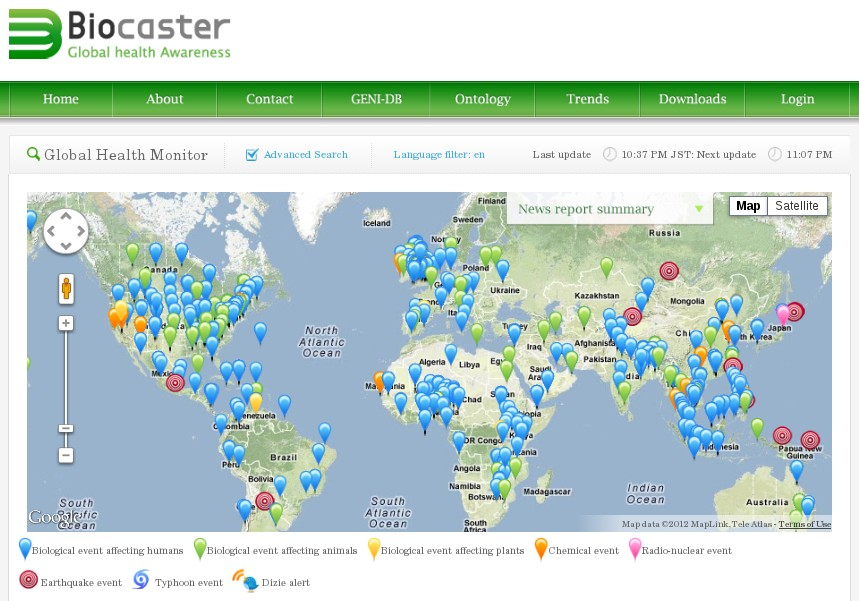
\includegraphics[width=1\textwidth, height=2.5in]{bio}
		\caption{\textbf{Hệ thống BioCaster}}
		\label{fig:bio}
\end{figure}

\begin{figure}[htbp]
		\centering
		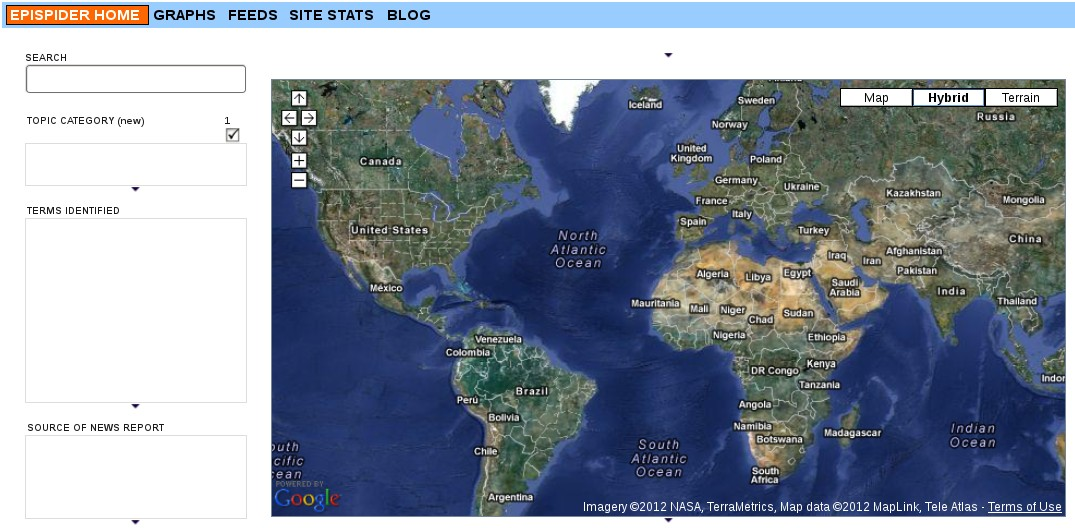
\includegraphics[width=1\textwidth, height=2in]{epi}
		\caption{\textbf{Hệ thống EpiSpider}}
		\label{fig:epi}
\end{figure}


\begin{figure}[htbp]
		\centering
		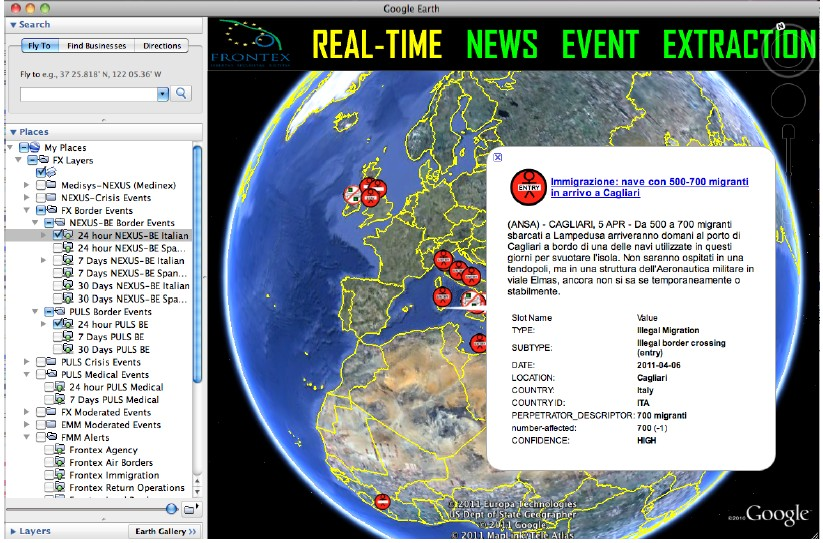
\includegraphics[width=1\textwidth]{frontex}
		\caption{\textbf{Hệ thống Frontex}}
		\label{fig:frontex}
\end{figure}


\begin{figure}[htbp]
		\centering
		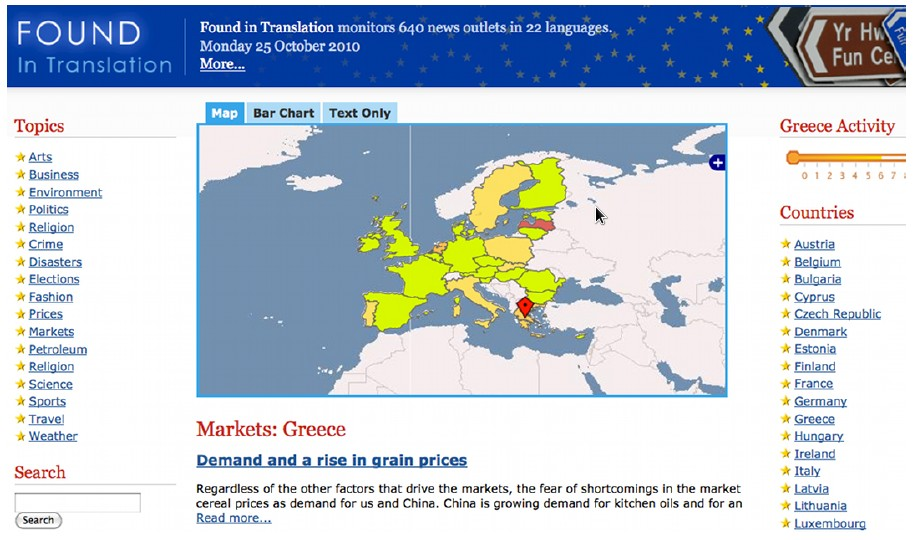
\includegraphics[width=1\textwidth]{noam}
		\caption{\textbf{Hệ thống NOAM}}
		\label{fig:noam}
\end{figure}




%Nghiên cứu của Hung cùng cộng sự lại là sự kết hợp giữa \emph{mẫu %lexico--syntactic} và phương pháp gán nhãn \emph{semantic role labeling}.

	\subsection{Một số nghiên cứu liên quan ở trong nước}
\noindent Trong khi bài toán trích xuất sự kiện trên thế giới đã có nhiều thành tựu đáng kể thì ở trong nước, trích xuất sự kiện vẫn là một bài toán mới mẻ. Tất cả các nghiên cứu của một số nhóm như nhóm do PGS.TS Đinh Điền (Đại học Khoa học Tự nhiên, Đại học Quốc Gia Thành Phố Hồ Chí Minh) chủ trì  đều chỉ dừng lại ở mức thử nghiệm phương pháp chứ chưa có công bố chính thức nào.
    \section{Tóm lược chương}


% ----------------------------------------------------------------------
